The robotic workcell consists of several subsystems: the storage station, the robot unit, the unloading station and bending machine terminal operating robot.
\begin{figure}[h]
    \centering
    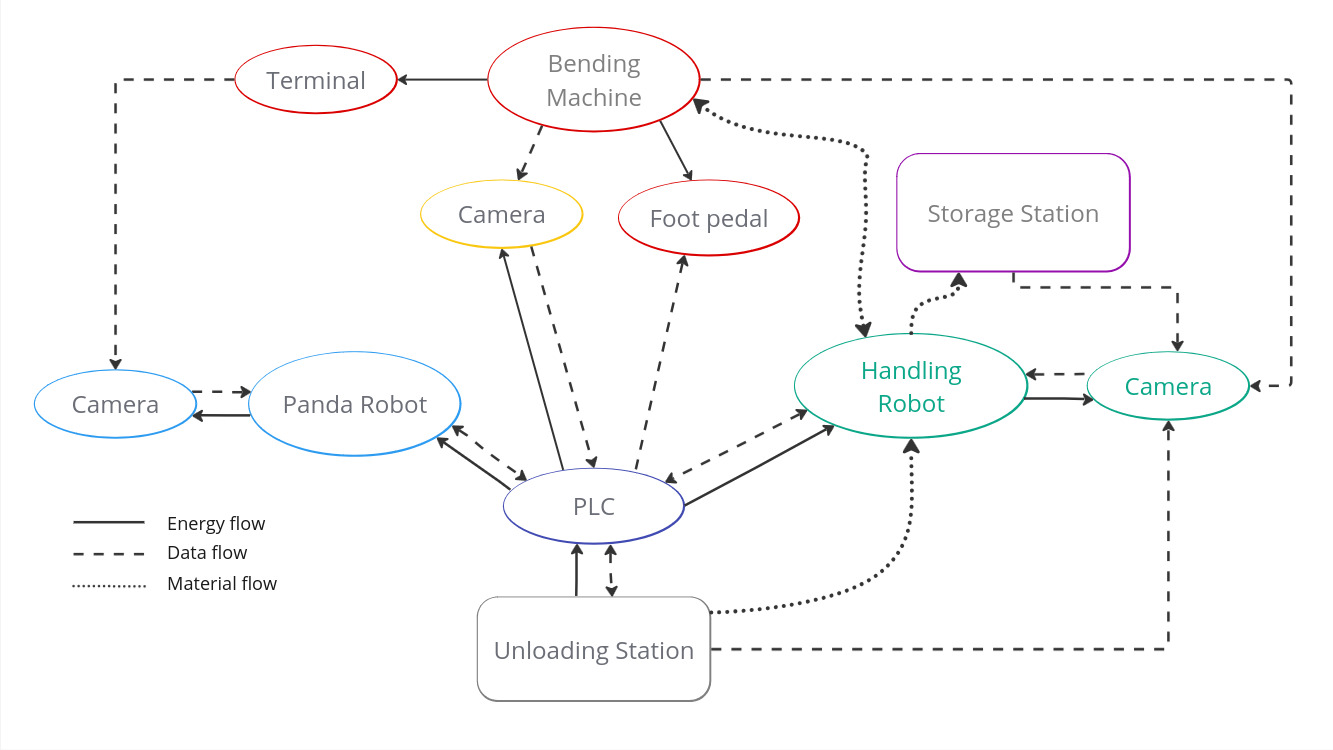
\includegraphics[width=\textwidth]{figures/workcell-flow.jpg}
    \caption{Energy, data and material flow in the robotic workcell}
    \label{fig:flow-workcell}
\end{figure}

Robotic workcell has been designed keeping in mind the handling robot workspace. Handling robot has been able to reach every station in the workspace without any collision. The drawers of storage system is especially close to the floor and the robot requires
some space to move around without getting stuck. Figure \ref{fig:robotic-workcell} shows the layout of the workcell. The robotic workcell consists of various subsystems which include:
\begin{itemize}
    \item Bending
\end{itemize}

The preliminary designs for the mobile robot unit were further elaborated
in the form of CAD models and successively converted into final CAD designs. Figure 1 shows the
current status of the mobile robot unit. This consists of several subsystems: the storage box, the robot
unit, the removal station, the VisCheck operating unit and the safety fence. The latter is still in the
preliminary design phase. The other subsystems are described in more detail in the following
subsections.

\begin{figure}[h]
    \centering
    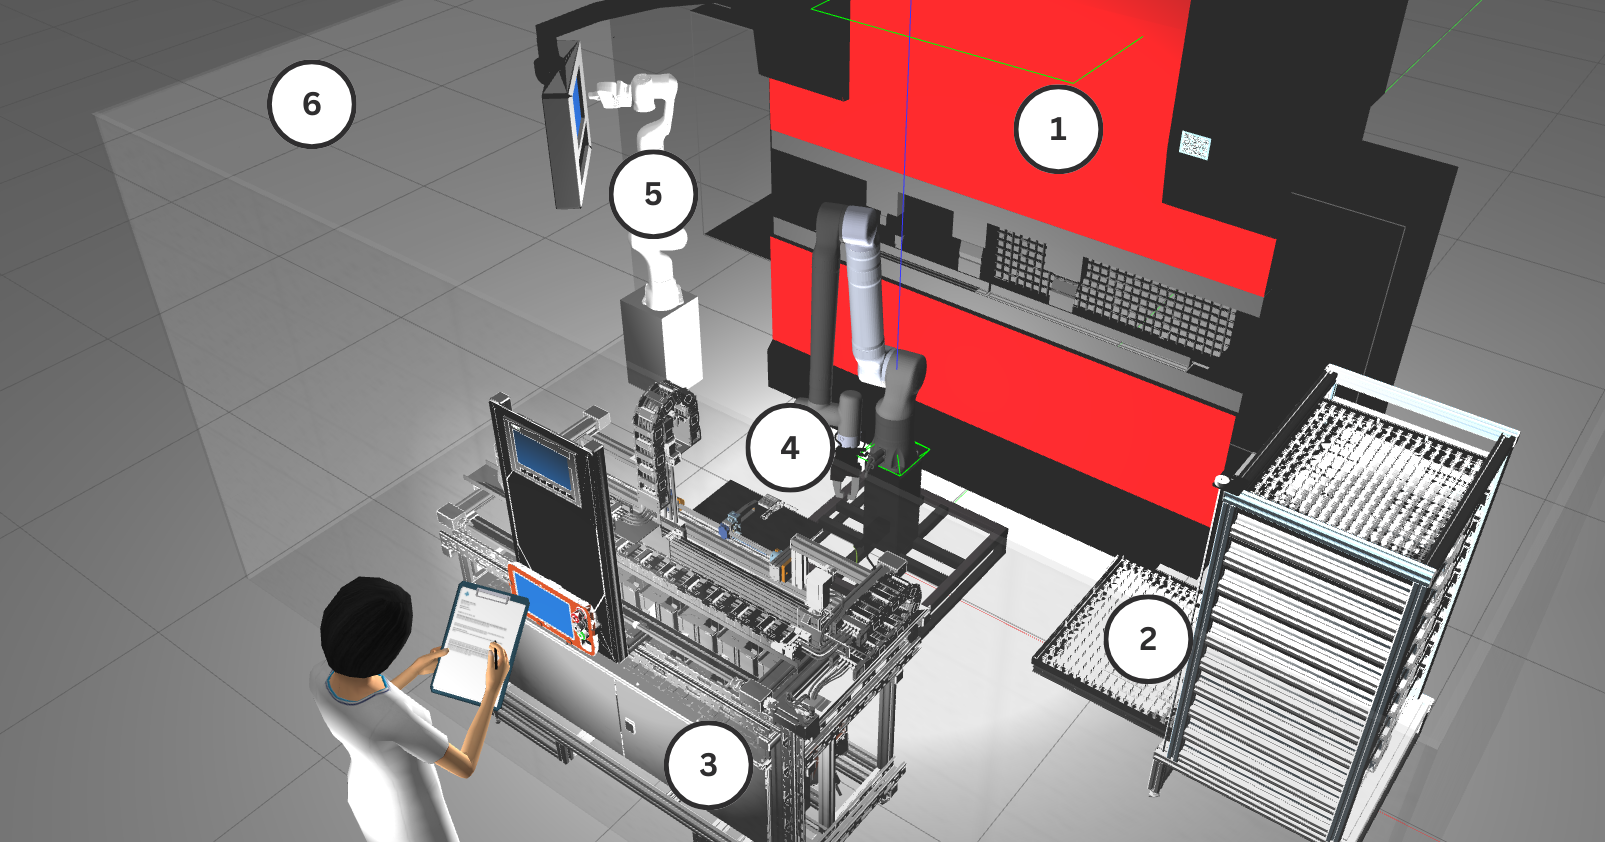
\includegraphics[width=\textwidth]{figures/robotic-workcell1.png}
    \caption{Robotic workcell layout. 1) Bending machine 2) Storage station 3) Unloading station 4) Handling robot 5) Bending machine terminal operating robot 6) Safety fence}
    \label{fig:robotic-workcell}
\end{figure}

